\subsection{Higgs physics at LHC}
\label{higgs}

One important physics purpose of LHC is searching for Higgs boson, which was the last missing part in SM.
This section will talk about both the production and decay modes of SM Higgs boson in proton-proton collision.

%% ================================ Higgs production ===============================
\textbf{Higgs productions}

Higgs boson can be produced through several processes.
There are 4 main production modes at LHC: gluon-gluon fusion (\textit{ggF}), vector boson fusion (\textit{VBF}),
associated production with vector-bosons (also called Higgs strahlung) (\textit{VH}) 
and associated production with a pair of top/antitop quarks (\textit{ttH}) \cite{Grojean:2243593}.
Figure~\ref{fig:higgs_productions_fd} shows the corresponding Feynman diagrams of each process (at LO).
\begin{figure}[!htb]
  \centering
  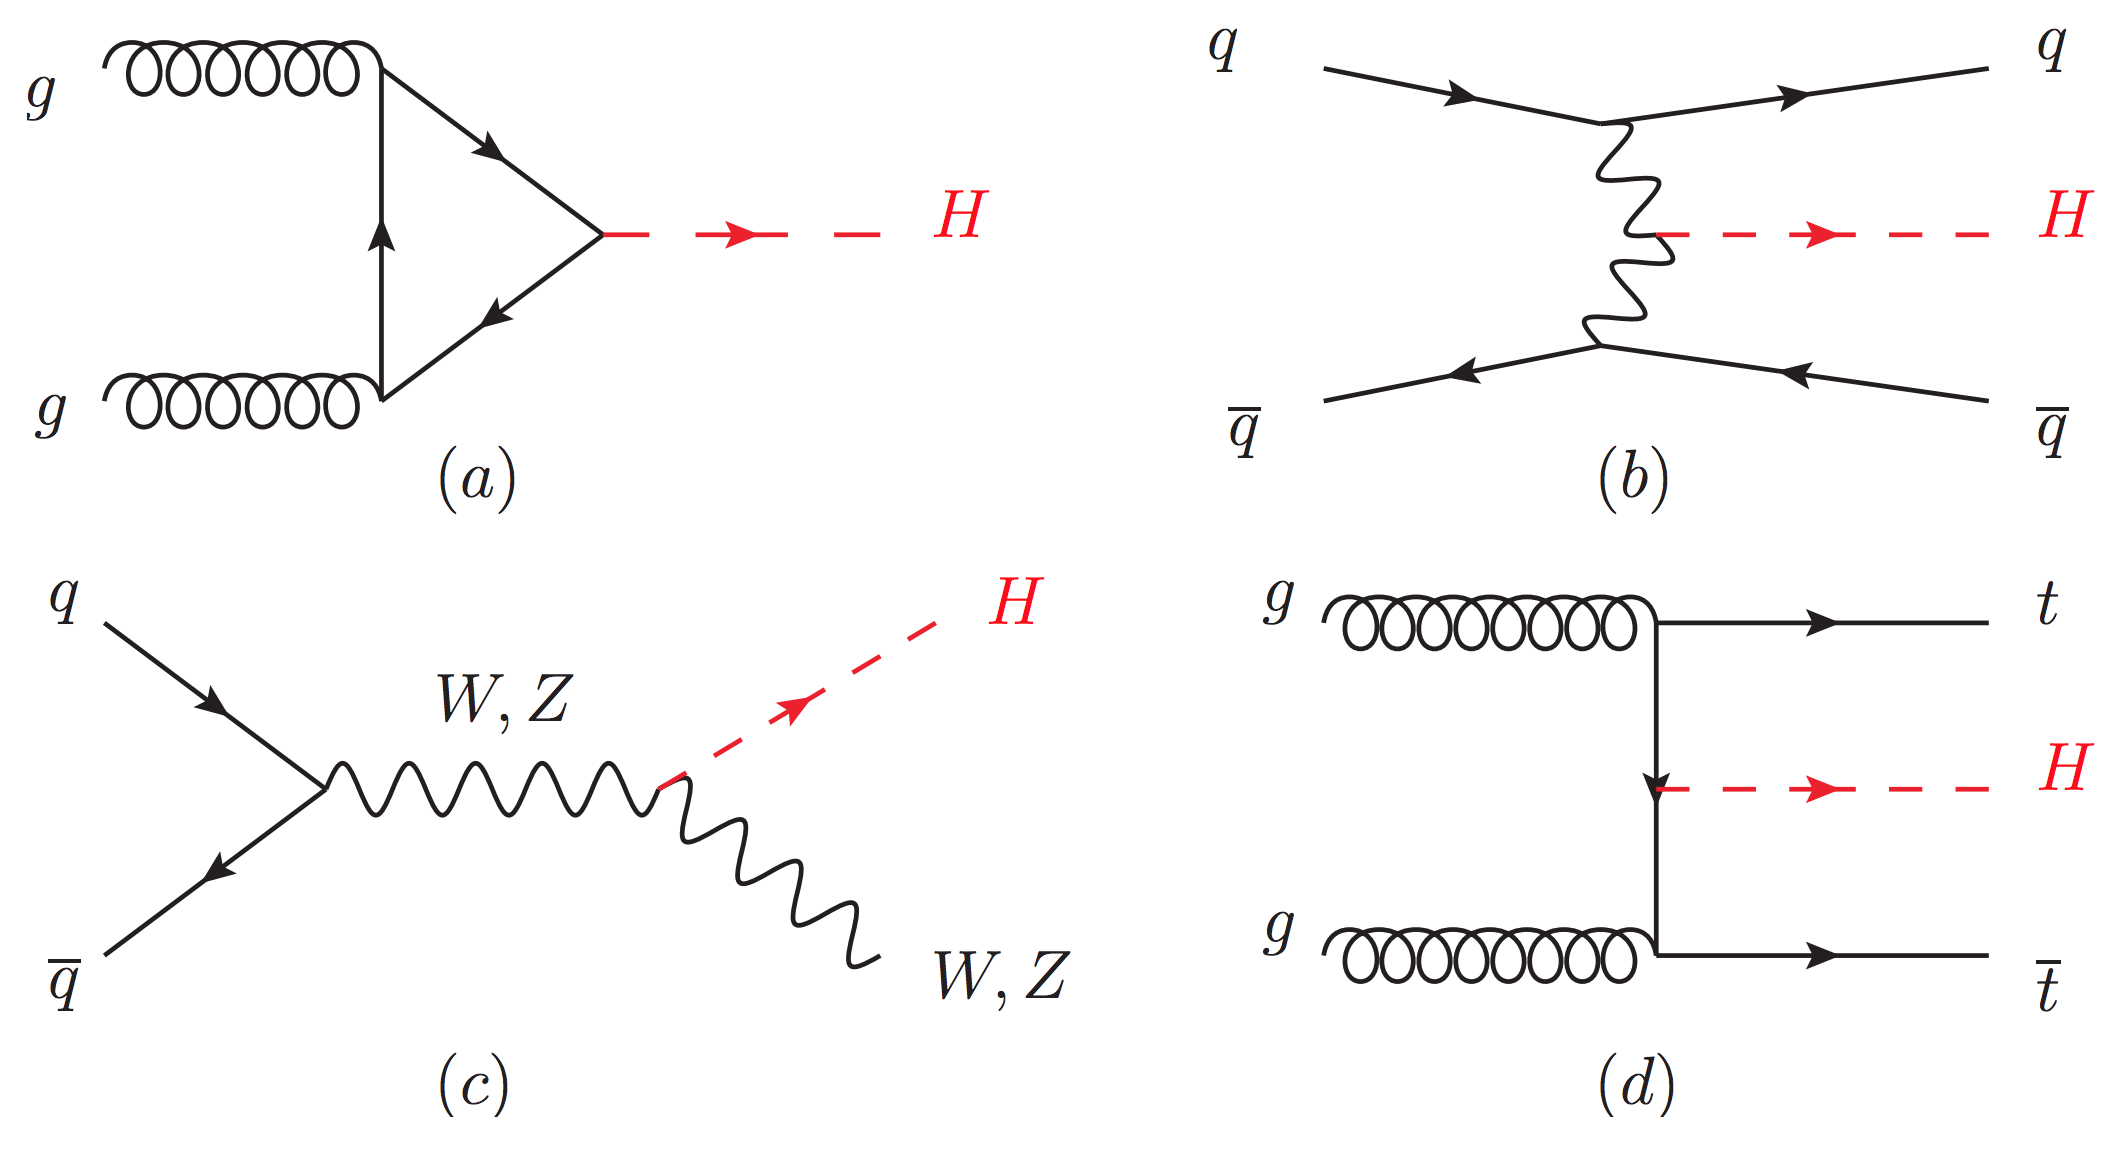
\includegraphics[width=0.8\textwidth]{figures/Theory/Figures_FeynmanHprod.png}
  \caption{Feynman diagrams of the Higgs production modes:
	   (a) ggF; (b) VBF; (c) VH; (d) ttH.}
  \label{fig:higgs_productions_fd}
\end{figure}
For pp collision, the cross section of productions of Higgs boson is as a function of center-of-mass-energy $\sqrt{s}$. 
Figure~\ref{fig:higgs_productions_xs} summarizes the cross section for SM Higgs with mass of 125 GeV.\\
\begin{figure}[!htb]
  \centering
  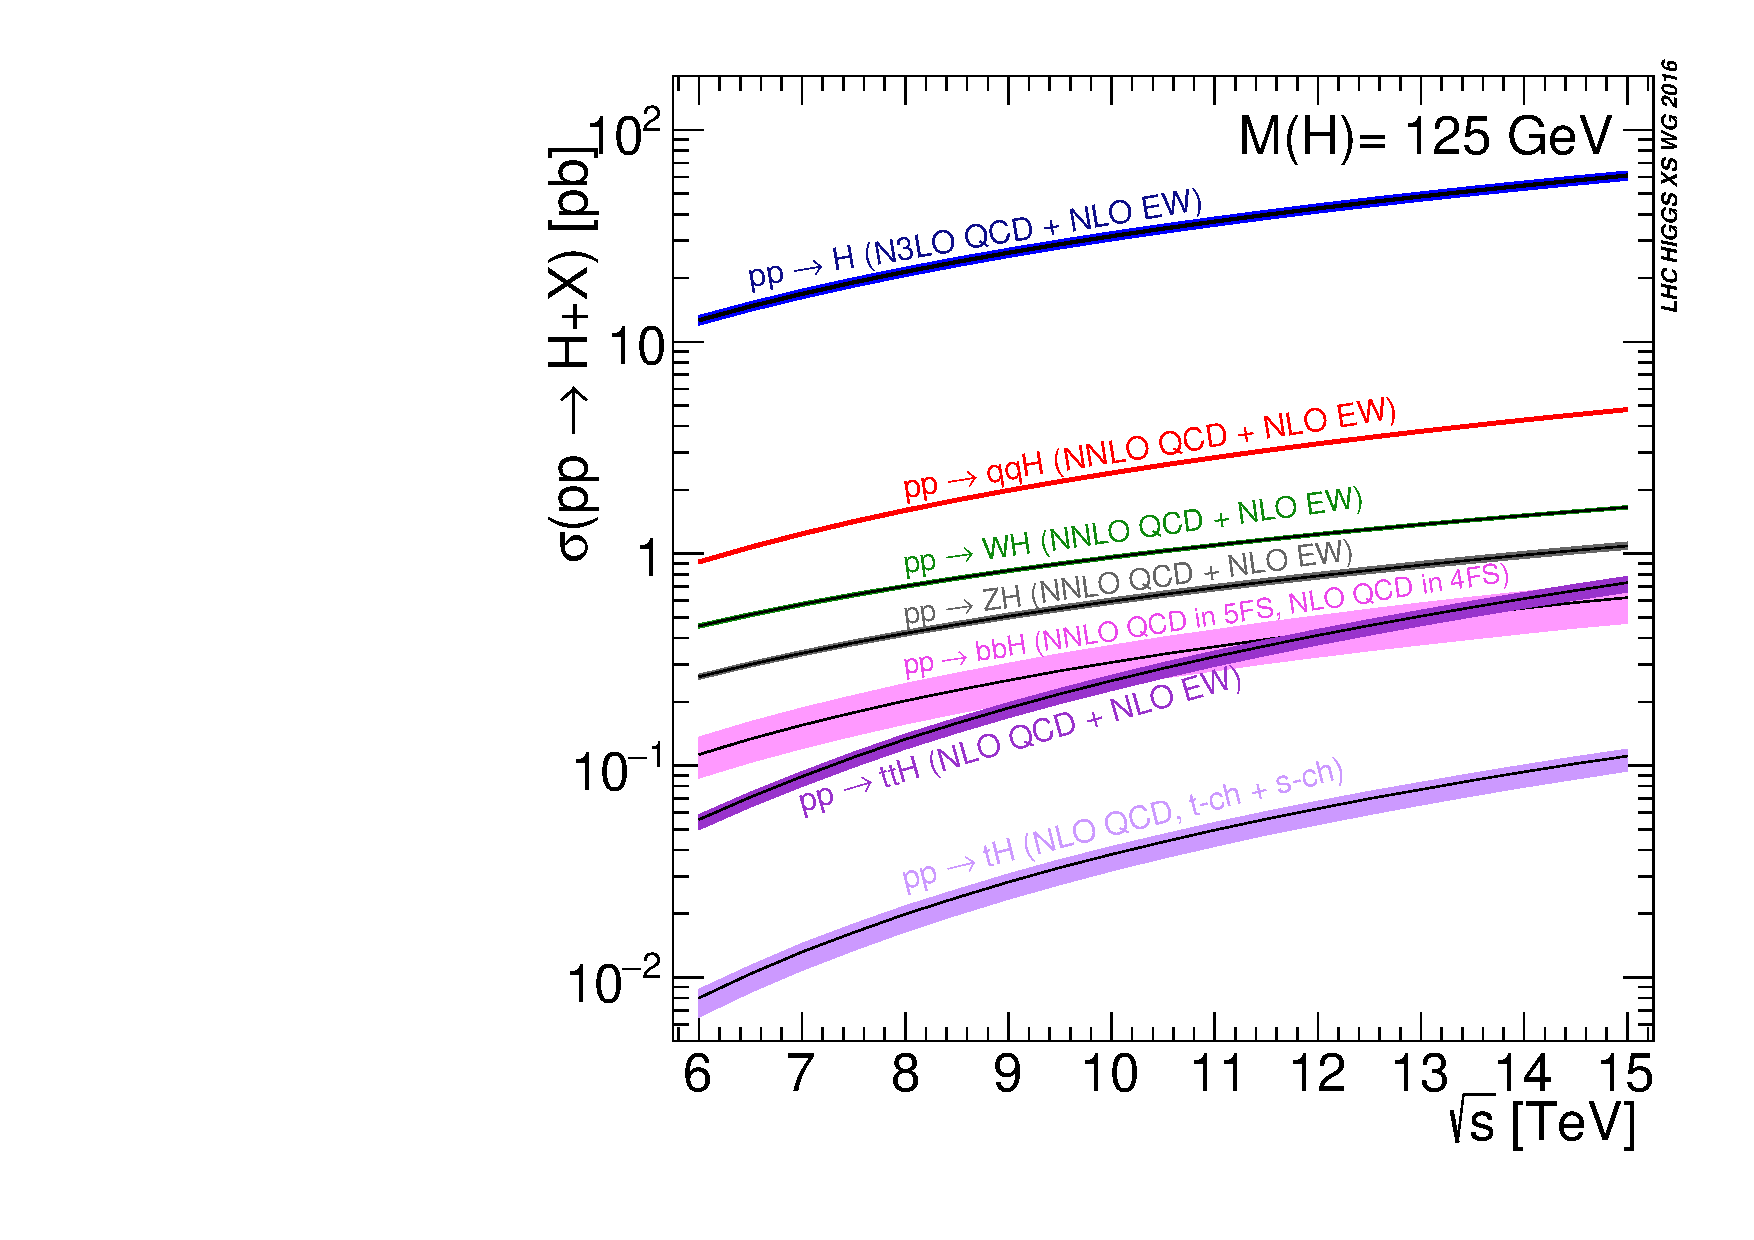
\includegraphics[width=0.5\textwidth]{figures/Theory/Plot_Escan_H125_new_sqrt.pdf}
  \caption{The SM Higgs boson production cross sections as a function of the center-of-mass-energy for pp collision.}
  \label{fig:higgs_productions_xs}
\end{figure}
Figure~\ref{fig:higgs_productions_xs2} summarizes the prospect of different Higgs boson production cross sections 
as a function of Higgs mass for pp collision center-of-mass-energy at 13 TeV and 14 TeV \cite{deFlorian:2227475}. 
\begin{figure}[!htb]
  \centering
  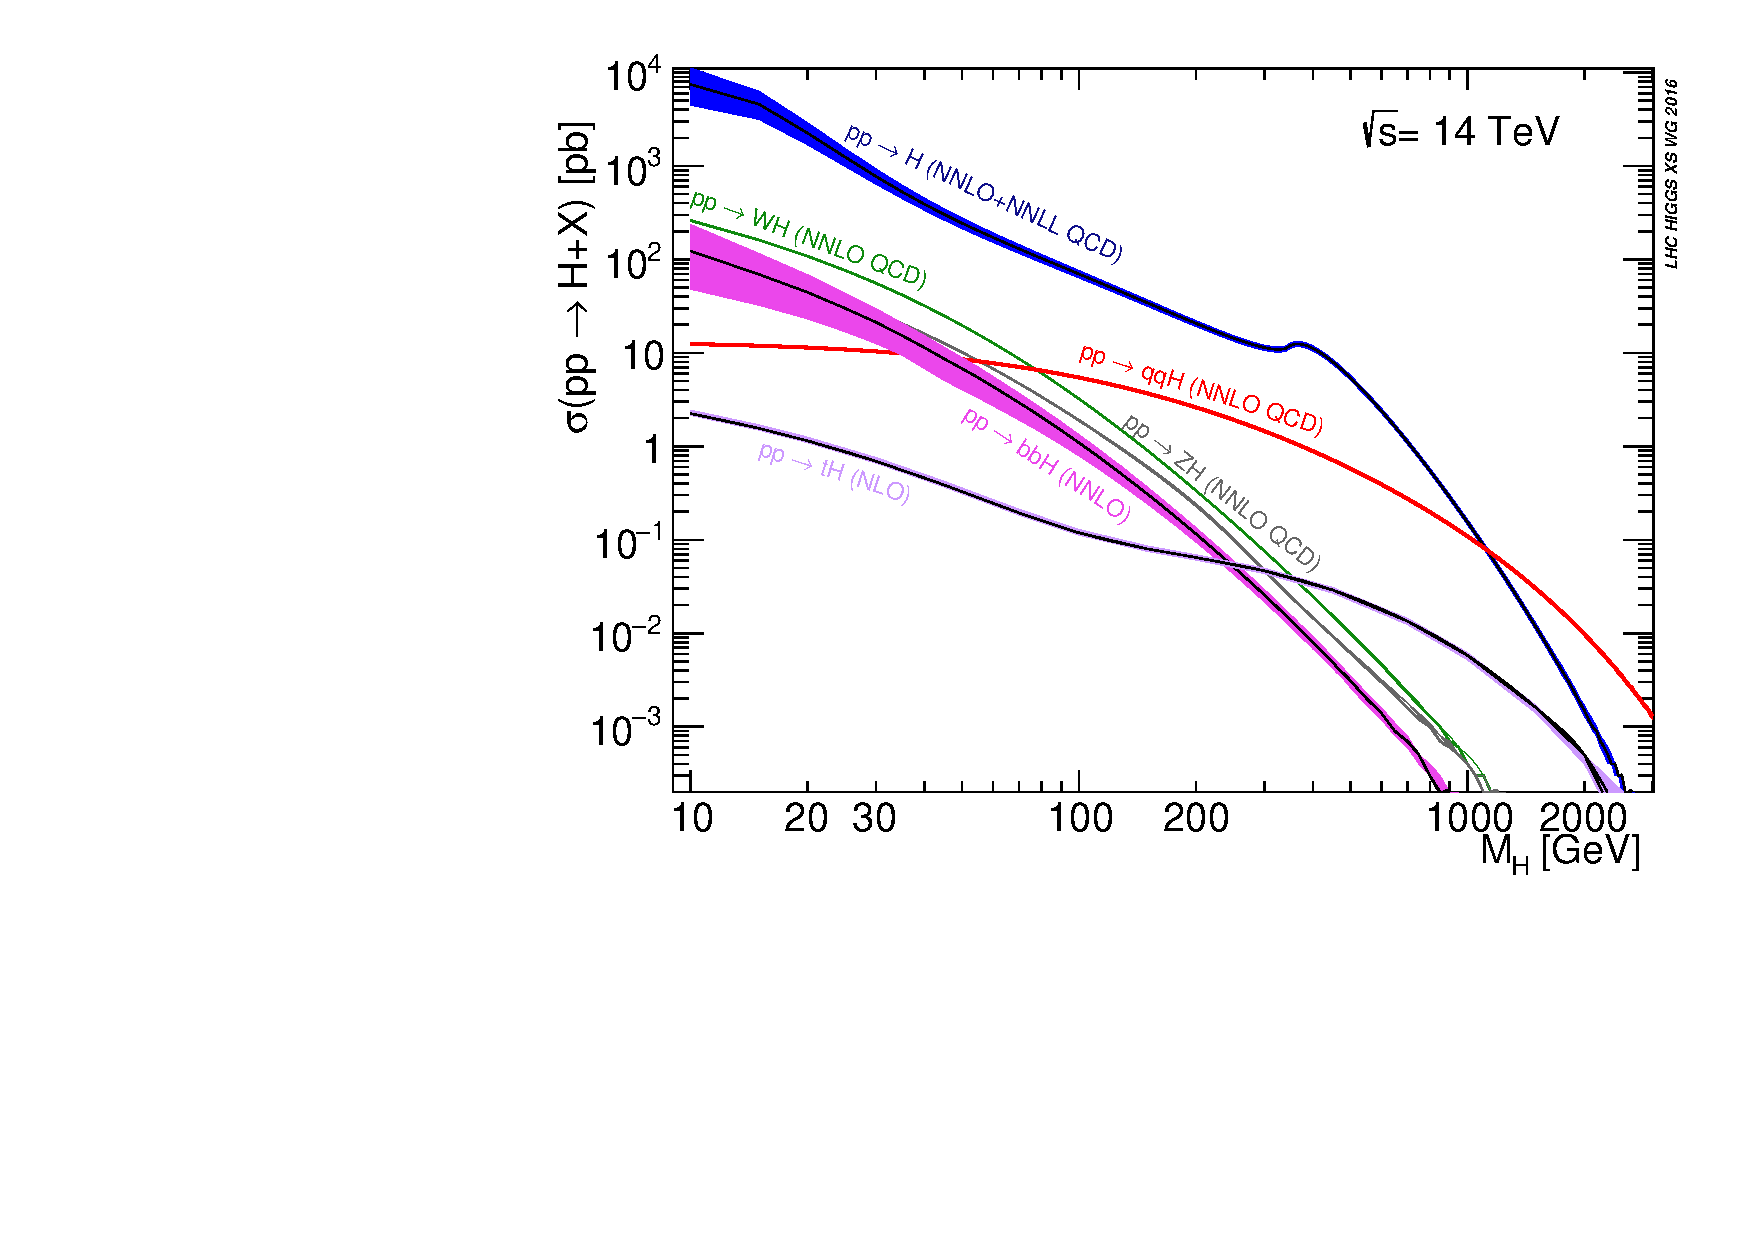
\includegraphics[width=0.45\textwidth]{figures/Theory/plotAll_14tev_BSM_sqrt.pdf}
  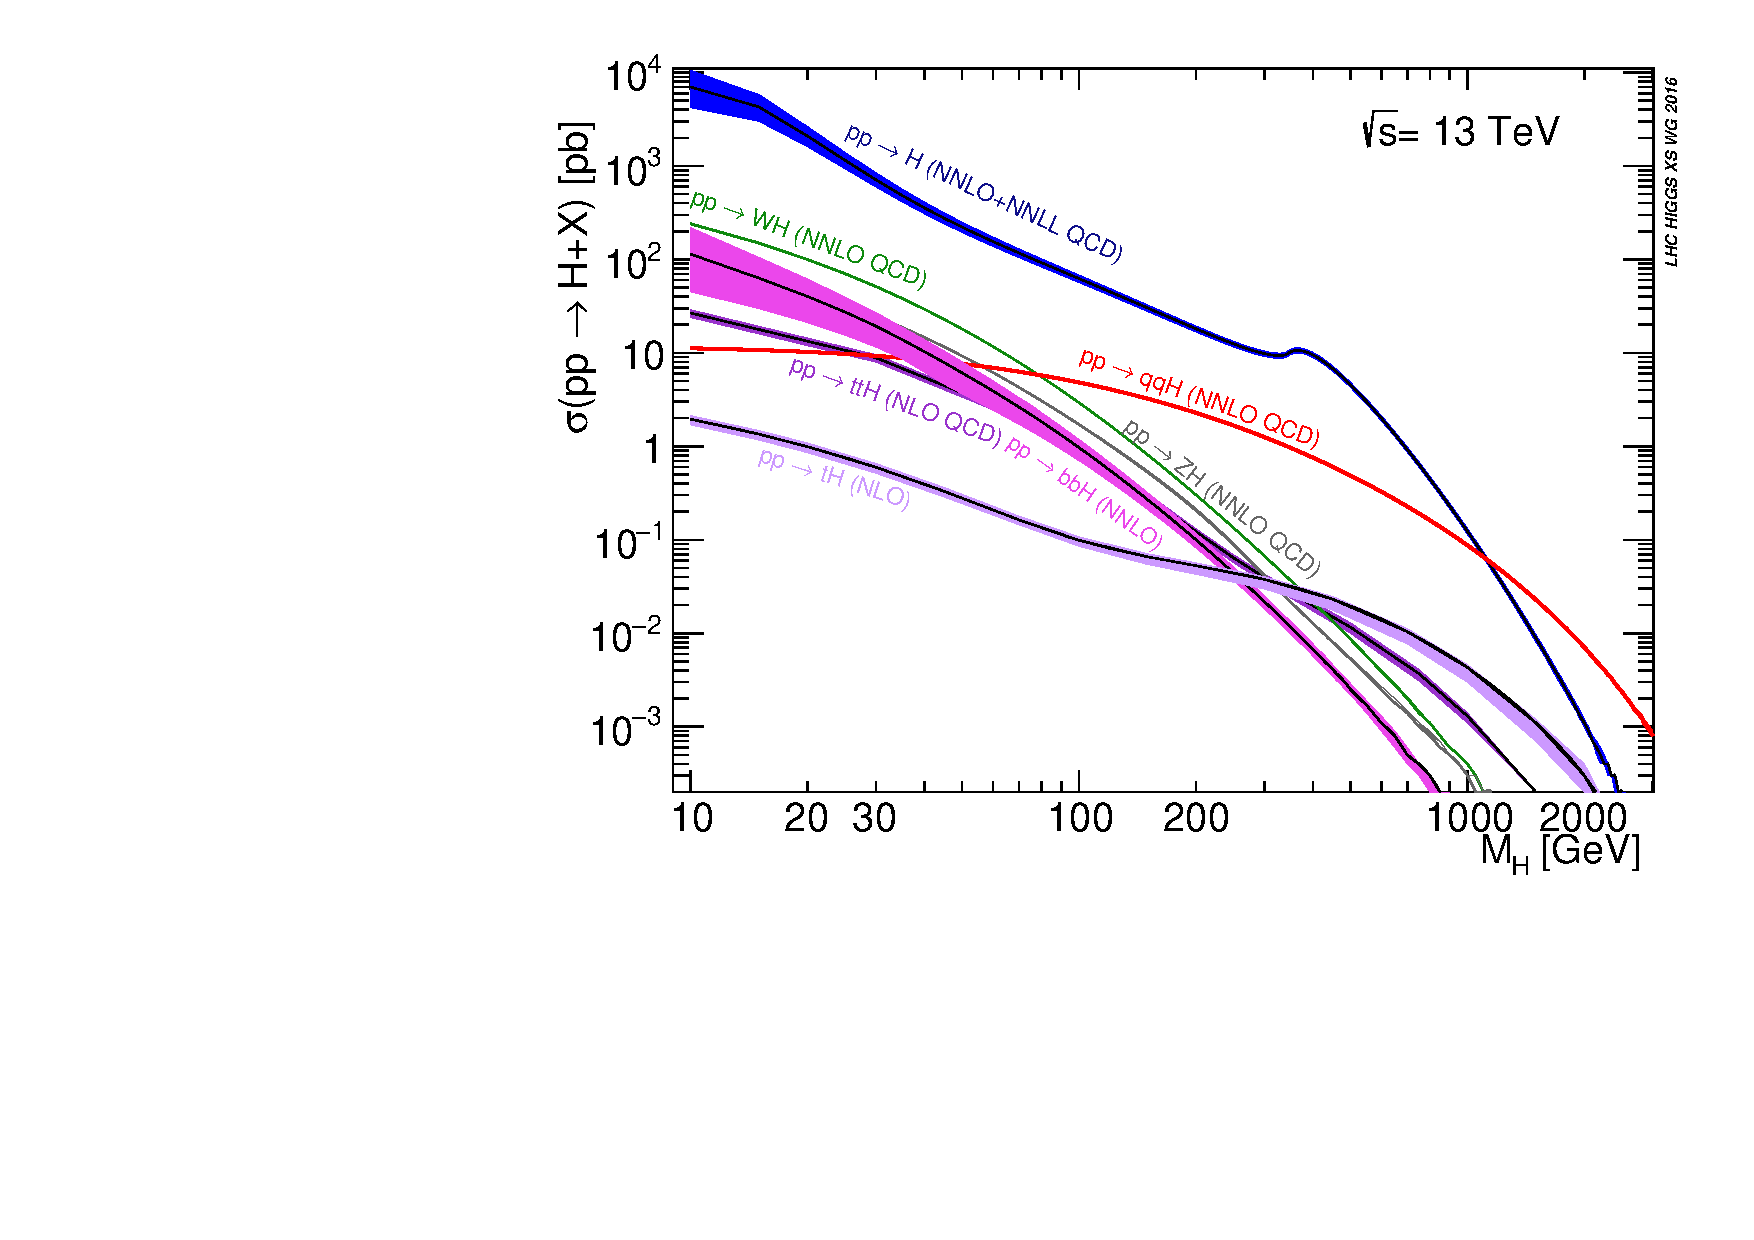
\includegraphics[width=0.45\textwidth]{figures/Theory/plotAll_13tev_BSM_sqrt.pdf}
  \caption{Higgs boson production cross section for various production modes as a function of the Higgs mass mH for $\sqrt{s}$ = 13 TeV (left) and 14 TeV (right) for pp collision.}
  \label{fig:higgs_productions_xs2}
\end{figure}

%% ================================ Higgs decays ===================================
\textbf{Higgs decays}

Higgs boson can interact with gauge bosons and fermions through gauge coupling and Yukawa coupling as introduced in section~\ref{symbreaking}.
Figure~\ref{fig:higgs_decay_fd} depicts Feynman diagrams of possible Higgs decay channels.
\begin{figure}[!htb]
  \centering
  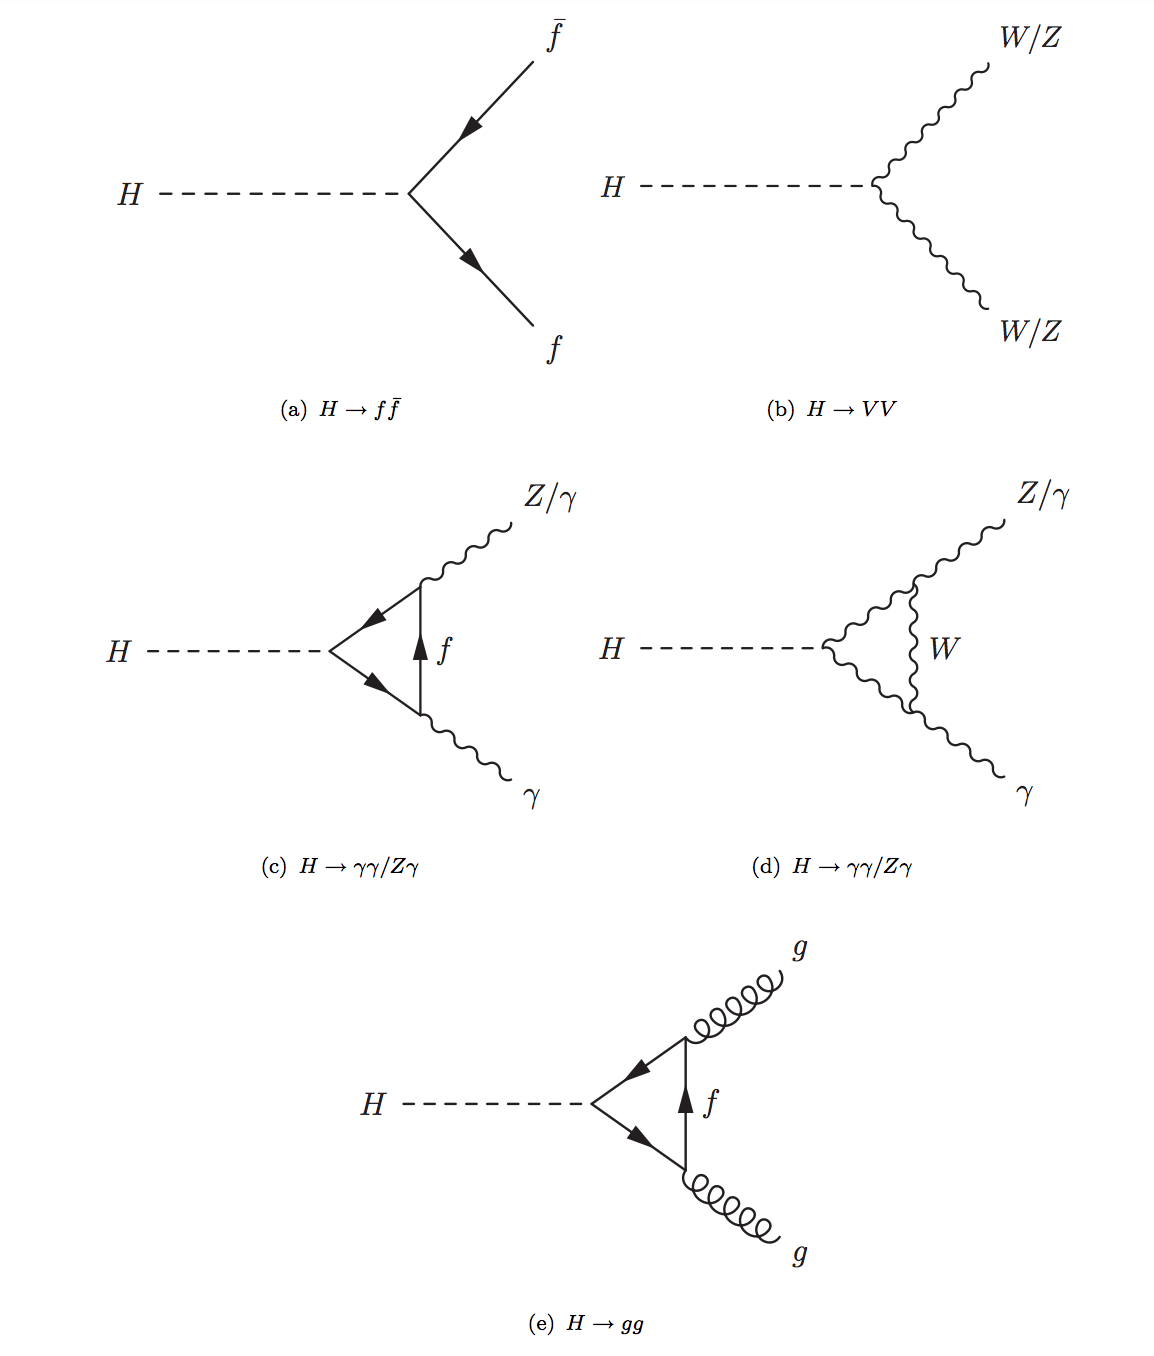
\includegraphics[width=0.8\textwidth]{figures/Theory/Figures_Feynman_Hdecay.png}
  \caption{SM Higgs decay channels.}
  \label{fig:higgs_decay_fd}
\end{figure}
The branching ratio of Higgs boson decaying into different final states as a function of Higgs mass is shown in figure~\ref{fig:higgs_decay_br}.
\begin{figure}[!htb]
  \centering
  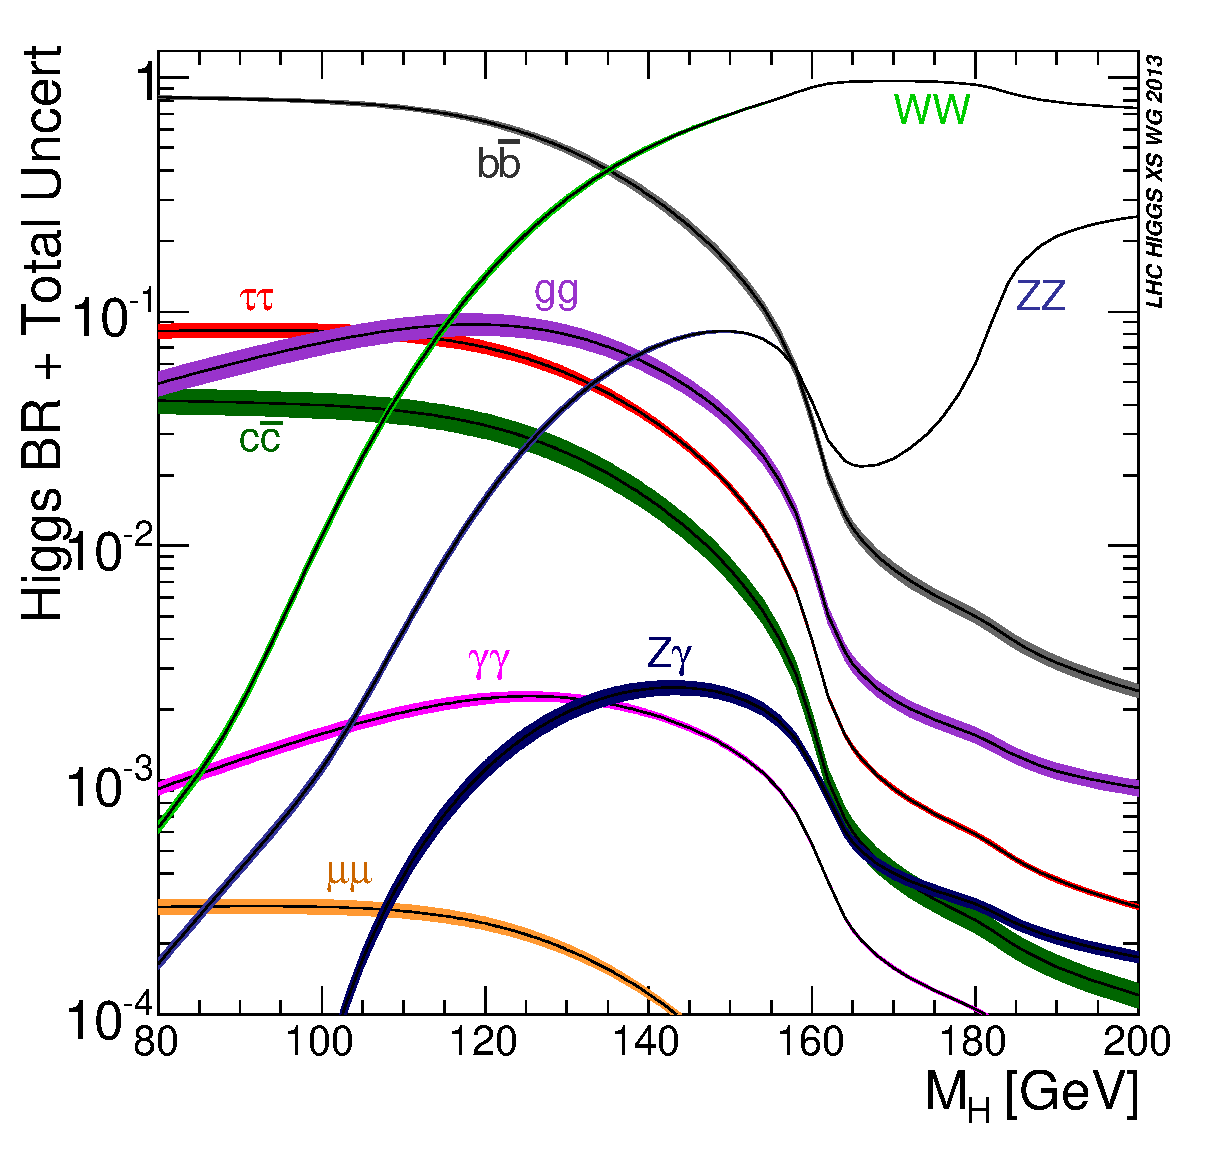
\includegraphics[width=0.5\textwidth]{figures/Theory/Higgs_BR_LM.eps}
  \caption{Branching ratio of Higgs decays \cite{Heinemeyer:1559921}. }
  \label{fig:higgs_decay_br}
\end{figure} 

%% ====================================== High mass related ===========================
\textbf{BSM Higgs models} 


